%\documentclass[]{beamer}
%\documentclass[handout]{beamer}
\documentclass[handout,draft]{beamer}

% Preambulo
% Paquetes para usar bien el idioma español
\usepackage[spanish,es-tabla]{babel}
\selectlanguage{spanish}
\usepackage[utf8]{inputenc}

% Paquetes para usar mejores imagenes
\usepackage{graphicx}

% Paquetes para links y tabla de contenidos en el PDF
\usepackage{hyperref}
\hypersetup{colorlinks=true,allcolors=blue}
%\usepackage{hypcap}

% Paquetes para mejores tablas
\usepackage{booktabs}

% Mejor matematica
\usepackage{amsmath}

% Fuentes de las imagenes
\usepackage[absolute,overlay]{textpos}

% Paquete captions
\usepackage[justification=centering,labelformat=empty,labelsep=none]{caption}

% Opciones para ticks
\usepackage{tikz}
\usetikzlibrary{shapes,arrows,positioning}

\tikzstyle{decision} = [diamond, draw, fill=blue!20, text width=4em, text badly centered, node distance=2cm, inner sep=0pt,on grid]
\tikzstyle{block} = [rectangle, draw, fill=blue!20, text width=8em, text centered, rounded corners, minimum height=2em,on grid]
\tikzstyle{line} = [draw, -latex]

% Citas bibliograficas
\usepackage[backend=biber]{biblatex}
\renewcommand{\footnotesize}{\tiny}
\addbibresource{biblio.bib}

% Mejoro las captions
\setbeamertemplate{caption}{\raggedright\insertcaption\par}

\setbeamertemplate{caption}{%
\begin{beamercolorbox}[wd=0.85\paperwidth, sep=.2ex]{block body}\insertcaption%
\end{beamercolorbox}%
}


% Sacar barra de navegacion
\setbeamertemplate{navigation symbols}{}%remove navigation symbols

% Transparencias en items
\setbeamercovered{transparent}

% Estilo de diapositivas
% \usetheme{Boadilla}
\usecolortheme{whale}
\usecolortheme{orchid}


\title{Herramientas de Teledetección Cuantitativa\\{\small Clase 7}}
\author{Francisco Nemi\~na}
\institute[Inst.]{
\includegraphics[height=1cm]{imagenes/logosopi.png}\phantom{pepe} 
\includegraphics[height=1cm]{imagenes/2mp.png}\phantom{pepe} 
\includegraphics[height=1cm]{imagenes/conae.png}}
\date{}
%\titlegraphic{
%\includegraphics[height=1cm]{IMAGENES/minplan.png}\phantom{1}
%
\includegraphics[height=1cm]{IMAGENES/conae.png}\phantom{1}
%
\includegraphics[height=1cm]{IMAGENES/sopi.png}}

\logo{
\includegraphics[height=0.7cm]{imagenes/sopi.png}}

\AtBeginSection[]
{
\begin{frame}
\frametitle{Esquema de presentaci\'on}
\tableofcontents[currentsection]
\end{frame}
}


\begin{document}
\begin{frame}
    \maketitle
\end{frame}
\section{Detecci\'on de cambios}
\subsection{Requisitos sobre las im\'agenes}
\begin{frame}{\subsecname}
  \begin{block}{Idea}
    Queremos poder detectar los patrones de cambio a partir de im\'agenes satelitales.
  \end{block}
\end{frame}
%--- Next Frame ---%

\begin{frame}{\subsecname}
  \begin{block}{Hip\'otesis}
    Vamos a suponer que cambios en las coberturas producen cambios en la radiometr\'ia.
  \end{block}
\end{frame}
%--- Next Frame ---%

\begin{frame}{\subsecname}
  \begin{block}{Requisitos}
    Las im\'agenes deben \pause
    \begin{itemize}[<+>]
      \item Estar corregidas radiometricamente.
      \item Estar corregistradas espacialmente.
    \end{itemize}
  \end{block}
\end{frame}
%--- Next Frame ---%

\subsection{M\'etodos basados en p\'ixeles}

\begin{frame}{\subsecname}
  \begin{block}{Diferencia de im\'agenes}
    Miramos la diferencia $$I_2 - I_1$$ para una banda y vemos como se distribuye
  \end{block}
\end{frame}
%--- Next Frame ---%

\begin{frame}{\subsecname}
  \begin{block}{Requisitos previos}
    Normalizando primero $$ \tilde{I_2} = \frac{\sigma_1}{\sigma_2} (I_2 - \mu_2) + \mu_1$$
  \end{block}
\end{frame}
%--- Next Frame ---%

\begin{frame}{\subsecname}
  \begin{block}{Diferencia de im\'agenes}
    Entonces $$\tilde{I_2} - I_1$$ es una distribuci\'on gaussiana entorno a cero relacionada con cuanto vario un p\'ixel.
  \end{block}
\end{frame}
%--- Next Frame ---%

\begin{frame}{\subsecname}
  \begin{figure}
  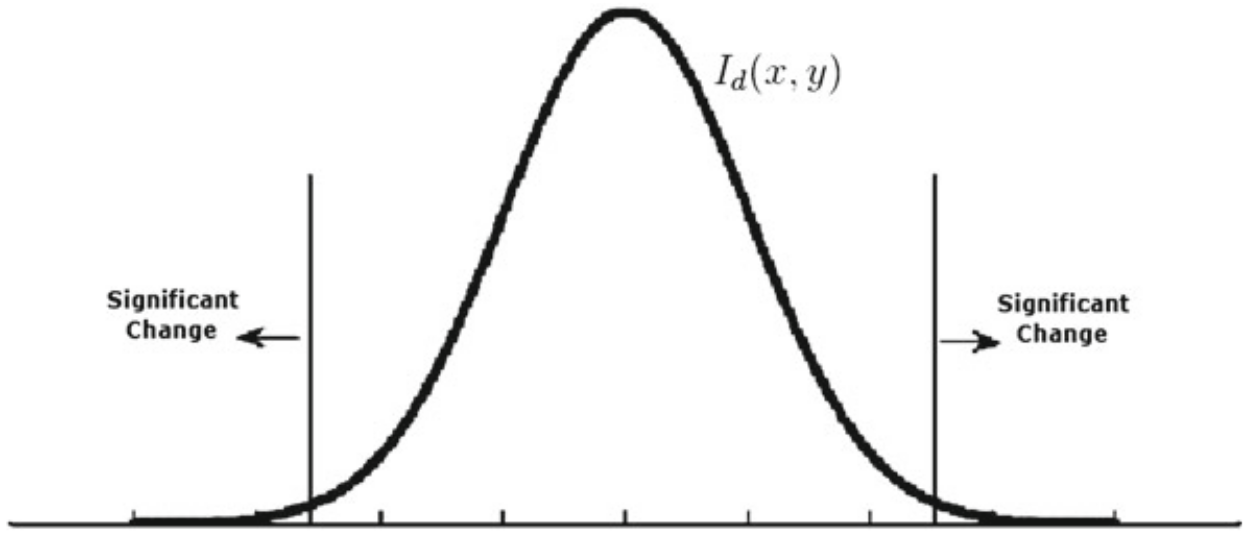
\includegraphics[width=0.6\textwidth]{imagenes/normal.png}
  \caption{Distribuci\'on de la diferencia entorno a cero.\footfullcite{unsalan2012two}}
  \end{figure}
\end{frame}
%--- Next Frame ---%

\begin{frame}{\subsecname}
  \begin{block}{Diferencia de im\'agenes}
    Decimos que encontramos cambio si la diferencia es mayor a cierto valor $\tau$. \pause ¿C\'omo lo elegimos?
  \end{block}
\end{frame}
%--- Next Frame ---%

\begin{frame}{\subsecname}
  \begin{block}{Selecci\'on de $\tau$}
    Existen varias formas de seleccionar $\tau$. En el caso particular que $$\tau = A \sigma$$ es posible calcular la probabilidad de que un p\'ixel este mal clasificado.
  \end{block}
\end{frame}
%--- Next Frame ---%

\begin{frame}{\subsecname}
  \begin{block}{Error en la detecci\'on}
    Para el caso anterior y bajo la suposici\'on gaussina, la probabilidad de que un p\'ixel sea incorrectamente clasificado como cambio es $$1 - \frac{2}{\sqrt\pi} \int_0^{A/\sqrt{2}\sigma} \exp(-y^2) dy$$
  \end{block}
\end{frame}
%--- Next Frame ---%

\begin{frame}{\subsecname}
  \begin{figure}
  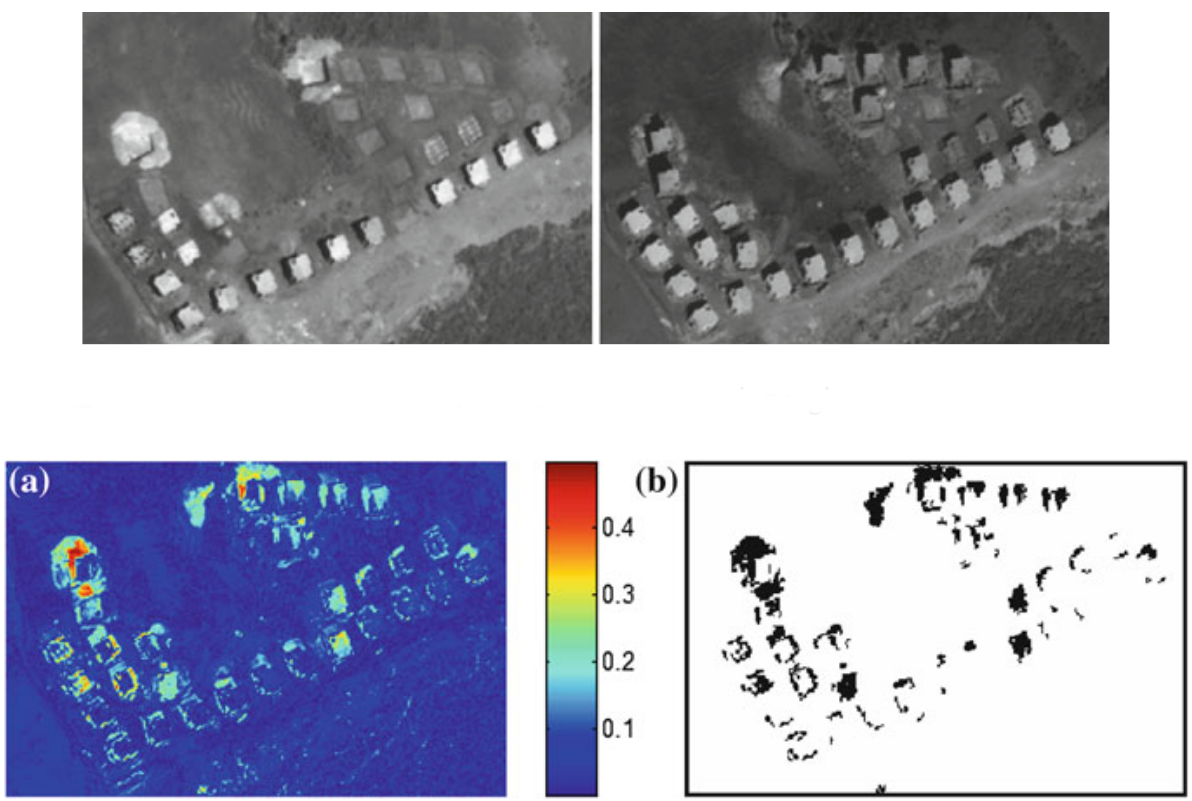
\includegraphics[width=0.8\textwidth]{imagenes/change.png}
  \caption{Zonas de cambio y no cambio para una banda.\footfullcite{unsalan2012two}}
  \end{figure}
\end{frame}
%--- Next Frame ---%

\begin{frame}{\subsecname}
  \begin{block}{Mas de una banda}
    Podemos plantear tambien diferencias entre bandas y obtener un vector de diferencias.
  \end{block}
\end{frame}
%--- Next Frame ---%

\begin{frame}{\subsecname}
  \begin{figure}
  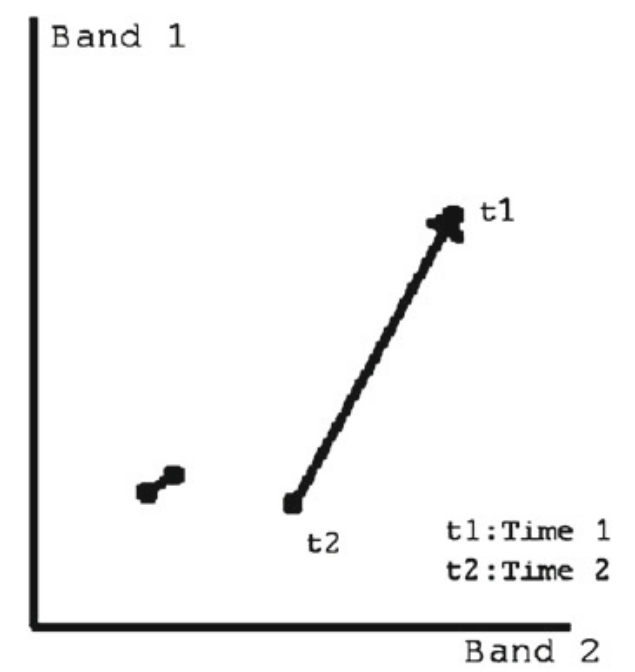
\includegraphics[width=0.5\textwidth]{imagenes/dvector.png}
  \caption{Vectores de diferencia.\footfullcite{unsalan2012two}}
  \end{figure}
\end{frame}
%--- Next Frame ---%

\begin{frame}{\subsecname}
  \begin{block}{Algunas consideraciones}
    \begin{itemize}[<+>]
      \item El modulo del vector de cambio se relaciona con la intensidad del mismo.
      \item Elegir si se trabaja con las bandas o una variable transformada es importante.
      \item Muchas veces no se analiza la variaci\'on de cada banda si no solo si la misma es positiva o negativa.
    \end{itemize}
  \end{block}
\end{frame}
%--- Next Frame ---%

\begin{frame}{\subsecname}
  \begin{figure}
  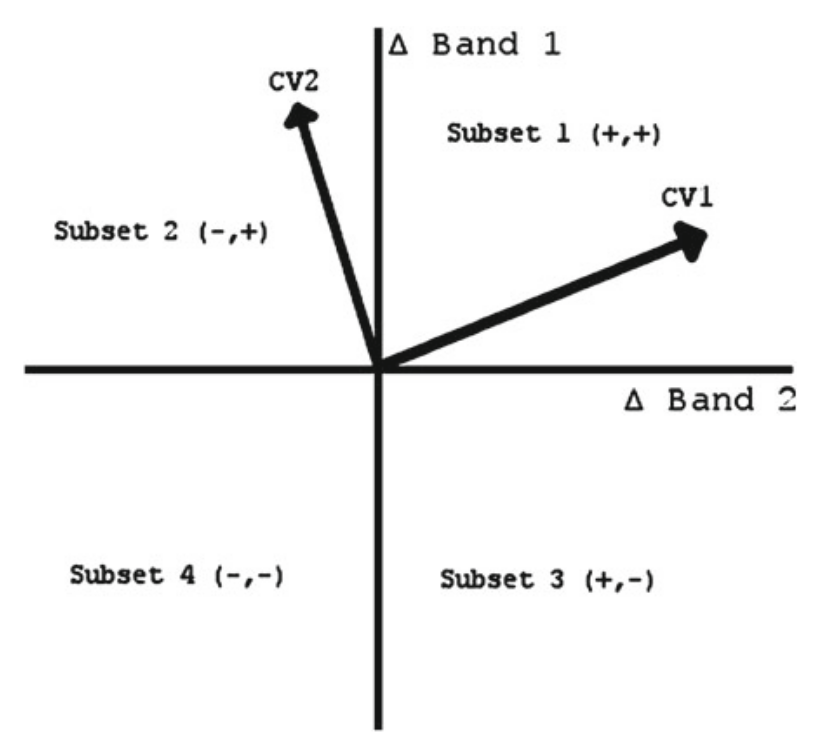
\includegraphics[width=0.5\textwidth]{imagenes/dangulos.png}
  \caption{Segmentaci\'on del espacio de bandas en zonas.\footfullcite{unsalan2012two}}
  \end{figure}
\end{frame}
%--- Next Frame ---%

\begin{frame}{\subsecname}
  \begin{block}{Detecci\'on de cambios por clasificaciones}
    Podemos detectar cambios en la imagen a partir de clasificaciones.\pause
    \begin{itemize}[<+>]
      \item Clasificar ambas im\'agenes.
      \item Encontrar que categorias cambian y en que zonas.
      \item Construya la matriz de probabilidad de cambio.
    \end{itemize}
  \end{block}
\end{frame}
%--- Next Frame ---%

\begin{frame}{\subsecname}
  \begin{figure}
  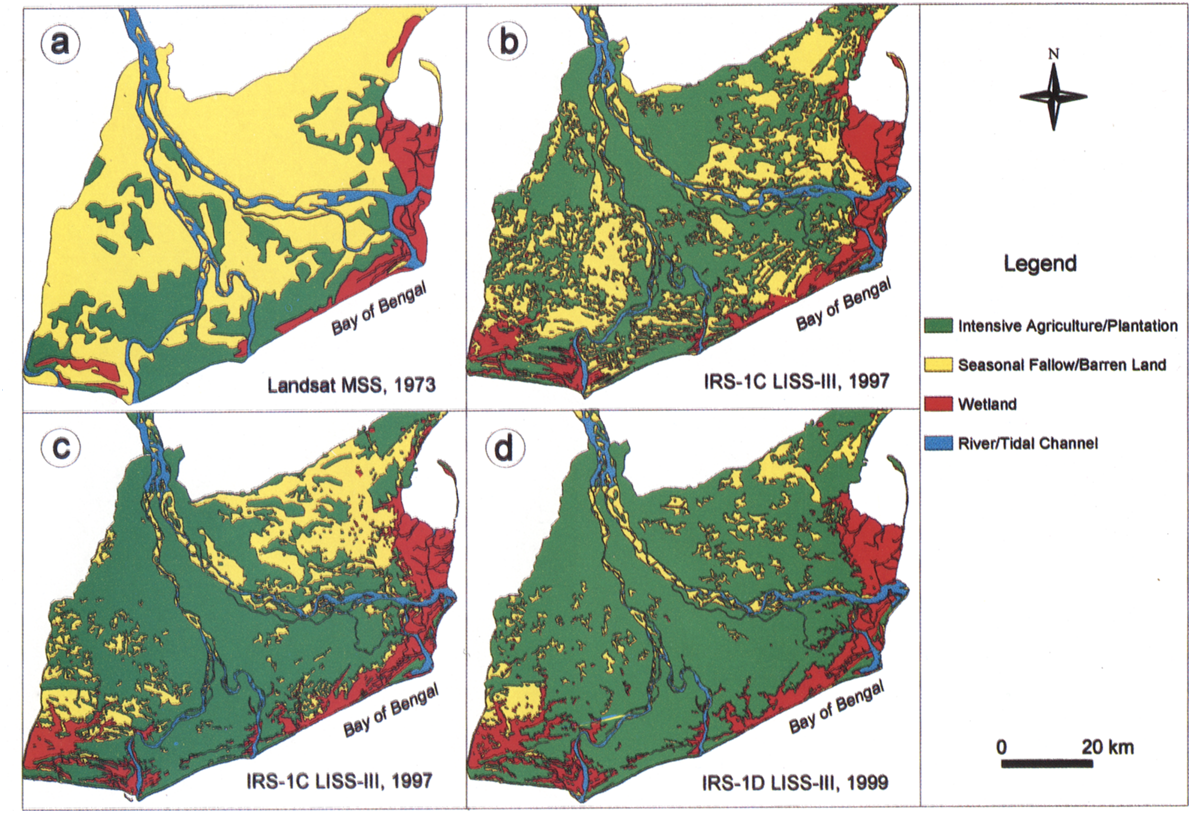
\includegraphics[width=0.8\textwidth]{imagenes/mapa_d.png}
  \caption{Cambios vistos a partir de una clasificaci\'on.\footfullcite{sarma2001landuse}}
  \end{figure}
\end{frame}
%--- Next Frame ---%

\begin{frame}{\subsecname}
\begin{block}{Definici\'on}
\[
\begin{bmatrix}
      & 1               & 2           &  \dots     & k \\
    1 & p_{11}          & p_{12}      & \dots & n_{1k} \\
    2 & p_{21}          & p_{22}      & \dots & n_{2k}      \\
    \vdots  & \vdots & \vdots & \ddots      & \vdots   \\
    k & p_{k1}          & p_{k2} & \dots       & n_{kk}
\end{bmatrix} \]
\pause Donde $$p_{ij} = \frac{n_{ij}}{N}$$ es la probabilidad de que la categoria $j$ se convierta en categoria $i$.
\end{block}
\end{frame}

\subsection{M\'etodos basados en transformaciones}

\begin{frame}{\subsecname}
  \begin{block}{Analisis por componentes principales}
    Hay dos formas de aplicarlo
    \begin{itemize}
      \item Analizando los componentes de cada imagen por separado.
      \item Analizando los componentes de ambas imagenes juntas.
    \end{itemize}
    \pause Como siempre el problema es la interpretaci\'on.
  \end{block}
\end{frame}
%--- Next Frame ---%

\begin{frame}{\subsecname}
  \begin{figure}
  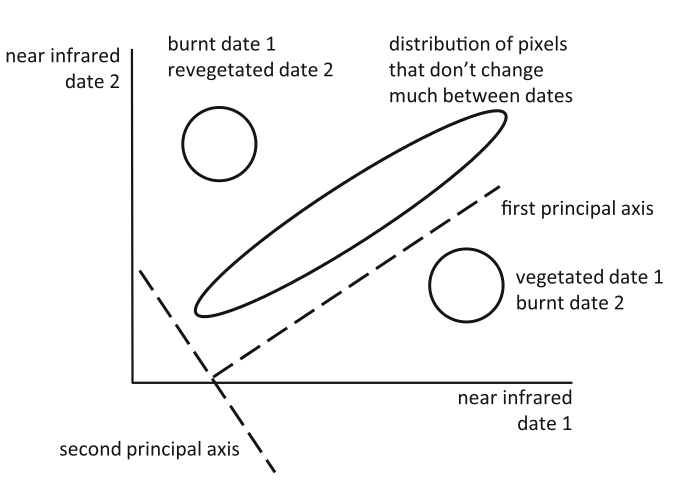
\includegraphics[width=0.8\textwidth]{imagenes/pca_cambio.png}
  \caption{Interpretaci\'on de componentes principales en una imagen.\footfullcite{richards2013remote}}
  \end{figure}
\end{frame}
%--- Next Frame ---%

\subsection{¿Que queda afuera?}

\begin{frame}{\subsecname}
  \begin{block}{Otras formas de de detecci\'on de cambio}
    \begin{itemize}[<+>]
      \item Transformada tasseled-cap
      \item \'Indices de vegetaci\'on
      \item Contextuales
    \end{itemize}
  \end{block}
\end{frame}
%--- Next Frame ---%

\section{Pr\'actica}

\begin{frame}{Pr\'actica}
  \begin{exampleblock}{Actividades pr\'acticas de la septima clase}
    \begin{enumerate}
      \item A partir de las im\'agenes LANDSAT de NDVI de febrero de los a\~nos 2004 y 2014 encuentre las zonas de aumento y disminuci\'on de la vegetaci\'on.
      \item A partir de las im\'agenes MODIS de NDVI de los a\~nos 2004 y 2014 encuentre las zonas de aumento y disminuci\'on de la vegetaci\'on.
      \item Calcule la matriz de probabilidad de cambio entre \'areas forestadas y no forestadas.
    \end{enumerate}
  \end{exampleblock}
\end{frame}
%--- Next Frame ---%

\end{document}
